\section{Experiment Details} \label{app:hyperparameter}

\subsection{Setup for CIFAR-10 Classification with WRN16-4 Model} \label{app:cifar}

In the paper, we have used CIFAR-10 classification task with wide residual network (WRN16-4) to demonstrate some points. To increase the reproducibility, we describe the detailed setting of these experiments.

We modify the standard WRN16-4~\citep{zagoruyko2016wide} following the suggestions of \cite{de2022unlocking}, i.e., replacing batch normalization with group normalization and using weight standardization for convoluntional weights, except that we do not use augmentation multiplicity for simplicity. Specifically, for flat clipping, \cite{de2022unlocking} uses a handed tuned clipping threshold $C=1$ and learning rate $\text{lr}=4$. Due to the fact that the learning rate and clipping thresholds jointly affect the performance in a complex way, we set the fixed per-layer clipping thresholds and the adaptive per-layer clipping thresholds so that they both have equivalent global threshold $C=1$. For fixed per-layer clipping, each layer clipping threshold is $C/\sqrt{K}$ where $K$ is the number of layers. For adaptive clipping thresholds $C_1, ..., C_K$, we rescale them $\tilde{C}_k := C \cdot C_k/\sqrt{\sum_k C_k^2}$ for all $k \in [K]$. 

To make the comparison more fair, we carefully tune the hyper-parameters of fixed per-layer clipping in Table \ref{table:fixed_global}, Table \ref{table:ablation_4_fixed_perlayer} and Figure \ref{fig:cifar_without_noise}. We find that small fixed thresholds can improve the performance of fixed per-layer clipping. We try different $C$'s from \{1.0, 0.5, 0.1, 0.05\} while making $C\cdot\text{lr}$ constant (which is critical for SGD), and set clipping threshold $C_k = C / \sqrt{K}$ for each layer. Finally, for fixed per-layer clipping, We choose the best hyper-parameter combinations ($C=0.05, \text{lr}=40$) and ($C=0.1, \text{lr}=20$) for $\epsilon=\{3,8\}$,  respectively.

For both fixed and adaptive per-layer clippings, we use the global strategy for noise allocation, i.e.,  $\gamma_k=1$ for all $k\in [K]$. Moreover, we use the same optimizer, weight decay, momentum, learning rate schedule, batch size and max epochs as flat clipping, as shown in Table \ref{tab:tuning_cifar10}. We tune the learning rate from two choices $\{2,4\}$ for all three algorithms. For adaptive per-layer clipping, we use a fraction $r=0.01$ of privacy budget to estimate quantiles and quantile learning rate $\eta=0.3$. We tune the target quantile from three choices $\{0.5, 0.6, 0.7\}$. We will evaluate the hyperparameter sensitivity in ablation study (Section \ref{app:ablation}).
Hyperparameters are tuned by training from scratch on training set and evaluating on test set. We use the best hyperparameter combinations for different $\epsilon$ respectively and report the test set accuracy of the last epoch in Table \ref{table:cifar_acc}.
 

 
\begin{table*}[ht]
\footnotesize
\setlength\tabcolsep{2.4pt}
\centering 
\caption{Hyper-parameters of flat clipping and per-layer clipping for WRN16-4 on CIFAR-10.} \label{tab:tuning_cifar10}
\begin{tabular}{l c c c}
\toprule
 & Adaptive per-layer & Fixed per-layer & Flat clipping \\
\midrule
\textbf{Optimizer} & \multicolumn{3}{c}{SGD} \\
\textbf{Weight Decay} & \multicolumn{3}{c}{0} \\
\textbf{Momentum} & \multicolumn{3}{c}{0} \\
\textbf{Learning Rate Schedule} & \multicolumn{3}{c}{Constant} \\
\textbf{Batch Size} & \multicolumn{3}{c}{4096} \\
\textbf{Max Epochs} & \multicolumn{3}{c}{300} \\
\midrule
\textbf{Learning Rate} & \{2, 4\} & equivalent \{2, 4\} & \{2, 4\} \\
\textbf{Allocation Method} & Global & Global & - \\

\textbf{Private Quantile Relative Budget $r$} & 1\% & - & -\\
\textbf{Quantile Learning Rate $\eta$} & 0.3 & - & -\\
\textbf{Target Quantile $q$} & \{0.5, 0.6, 0.7\} & - & - \\
\bottomrule
\end{tabular}
\end{table*}

 

\subsection{Setup for GLUE Tasks with RoBERTa Models } \label{app:glue}

To evaluate the performance of adaptive per-layer clipping, we conduct experiments on GLUE tasks by fine-tuning RoBERTa-base and RoBERTa-large models with differential privacy.

The optimizer setup and dropout rates are the same for adaptive per-layer clipping, fixed per-layer clipping, fixed flat clipping and adaptive flat clipping, as shown in Table \ref{tab:roberta_tuning_sst2}.

For per-layer clipping, we use the global strategy for noise allocation, i.e., $\gamma_k=1$ for all $k\in [K]$.

We tune other hyperparameters: peak learning rate, batch size, clipping thresholds for fixed per-layer clipping, target quantile $q$ for adaptive per-layer clipping, as shown in the bottom half of Table \ref{tab:roberta_tuning_sst2}.

To tune hyperparameters fairly, we split the training set of SST-2 into two parts: a new training set containing 80\% of original training set and a validation set containing the remaining. 
We select the best hyperparameters with the performance on the validation set, averaging over 3 different seeds. 
Table \ref{tab:roberta_tuning_sst2} shows the best hyperparameter combinations we use for adaptive and fixed per-layer clipping.

For experiments in Section~\ref{subsec:roberta}, we set the privacy budget for quantile estimation $r=10\%$. 
Figure \ref{fig:ablation-2-quantile-budget} suggests that using smaller values such as $r=1\%$ or $r=5\%$ may produce slightly better results.

We transfer hyperparameters tuned on SST-2 to the remaining GLUE tasks. Specifically, we follow \cite{li2022large} and keep the sampling rate the same across different datasets. 

For the GLUE tasks considered, we find that training for more epochs generally improves the performance for both flat and per-layer clipping. 
To ensure runs finish under realistic training times, we fix the max epochs to be 20 for experiments for the adaptive per-layer clipping runs reported in Table~\ref{table:glue}. 
We report the accuracies on the original dev sets for each GLUE task.

For the second experiment in Section~\ref{subsec:roberta}, we only optimize with respect to the self-attention layers and the classification head parameters for both flat clipping and adaptive per-layer clipping so that the total computational cost of this controlled ablation study is manageable.


\begin{table*}[ht]
\footnotesize
\setlength\tabcolsep{2.4pt}
\centering 
\caption{Hyper-parameters of per-layer clipping for RoBERTa on SST-2 dataset, where the \textbf{text in bold} denotes the hyper-parameters we eventually use.} \label{tab:roberta_tuning_sst2}
\begin{tabular}{l cc cc}
\toprule
\textbf{Model} & \multicolumn{2}{c}{RoBERTa-base} & \multicolumn{2}{c}{RoBERTa-large}  \\
\textbf{Method} & Adaptive & Fixed  & Adaptive & Fixed \\ 
\midrule
\textbf{Optimizer} & \multicolumn{4}{c}{Adam} \\
\textbf{Adam ($\beta_1$, $\beta_2$)} & \multicolumn{4}{c}{(0.9, 0.98)}   \\
\textbf{Adam $\epsilon$} & \multicolumn{4}{c}{$10^{-6}$}   \\ 
\textbf{Weight Decay} & \multicolumn{4}{c}{0}   \\ 
\textbf{Warm-up Ratio} & \multicolumn{4}{c}{0.06} \\ 
\textbf{Learning Rate Schedule} & \multicolumn{4}{c}{Linear Decay}   \\ 
\textbf{Dropout} & \multicolumn{4}{c}{0.1} \\ 
\textbf{Attention Dropout} & \multicolumn{4}{c}{0.1} \\ 
\textbf{Max Epochs} & \multicolumn{4}{c}{20} \\
\midrule
\textbf{Peak Learning Rate} & $\{1,\textbf{2},4\}\times10^{-4}$ & $\{\textbf{1},2,4\}\times10^{-4}$ & $\{1,\textbf{2},4\}\times10^{-4}$ & $\{1,\textbf{2},4\}\times10^{-4}$\\ 
\textbf{Batch Size} & $\{1,\textbf{2},4\}\times2^{9}$ & $\{\textbf{1},2,4\}\times2^{9}$ & $\{\textbf{1},2,4\}\times2^{9}$ & $\{\textbf{1},2,4\}\times2^{9}$  \\ 
\textbf{Allocation Method} & \multicolumn{4}{c}{Global} \\
\textbf{Init Threshold} & 1.0 & \{\textbf{0.1}, 0.5, 1.0\} & 1.0 & \{0.1, 0.5, \textbf{1.0}\} \\
\textbf{Private Quantile Relative Budget $r$} & 10\% & - & 10\% & - \\ 
\textbf{Quantile Learning Rate $\eta$} & 0.3 & - & 0.3 & - \\ 
\textbf{Target Quantile $q$} & \{0.5, 0.75, \textbf{0.85}\} & -  & \{0.5, 0.75, \textbf{0.85}\} & -  \\
\bottomrule
\end{tabular}
\end{table*}

\subsection{Setup for Language Generation Tasks with GPT-2} \label{app:lang_gen}

We reused most of the hyperparameters specific to adaptive quantile estimation based on tuning results on SST-2. 
We retuned the target quantile parameter as we observed that optimal values of this parameter tend to be different for different tasks. 
To ensure a fair comparison against full fine-tuning, we constrain the runs with adaptive per-layer clipping to have the same batch size and training epochs as in~\citep{li2022large}. 
We adopted the default values set by the Hugging Face \texttt{transformers}  library for Adam's $\beta_1$, $\beta_2$, and $\epsilon$. 
Table \ref{tab:gpt2_tuning} contains the full set of hyperparameters. 




\begin{table*}[ht]
\footnotesize
\setlength\tabcolsep{2.4pt}
\centering 
\caption{Hyperparameters for full fine-tuning GPT-2 with adaptive per-layer clipping. Numbers in bold are best performing hyperparameters used for reporting final results. 
} \label{tab:gpt2_tuning}
\begin{tabular}{l cc}
\toprule
\textbf{Model} & \multicolumn{2}{c}{GPT-2} \\
\textbf{Dataset} & E2E & DART \\ 
\midrule
\textbf{Optimizer} & \multicolumn{2}{c}{Adam} \\
\textbf{Adam ($\beta_1$, $\beta_2$)} & \multicolumn{2}{c}{(0.9, 0.999)}   \\
\textbf{Adam ($\epsilon$)} & \multicolumn{2}{c}{1e-8}   \\
\textbf{Weight Decay} & \multicolumn{2}{c}{0} \\
\textbf{Learning Rate Schedule} & \multicolumn{2}{c}{Linear Decay} \\
\textbf{Batch Size} & 1000 & 1500 \\
\textbf{Max Epochs} & 10 & 15 \\
\textbf{Learning Rate} & \multicolumn{2}{c}{$2 \times 10^{-3}$ } \\
\textbf{Allocation Method} & \multicolumn{2}{c}{Global} \\
\textbf{Init Threshold} & \multicolumn{2}{c}{0.01} \\
\textbf{Private Quantile Relative Budget $r$} & \multicolumn{2}{c}{1\%} \\
\textbf{Quantile Learning Rate $\eta$} & \multicolumn{2}{c}{0.3} \\
\textbf{Target Quantile $q$} & $\{\mathbf{0.3}, 0.5, 0.7, 0.9\}$ & reuse best of left \\
\bottomrule
\end{tabular}
\end{table*}



\section{Additional Experiments on Gradient Norm Shift}\label{app:gradnorm-shift}

In this section, we illustrate the distribution of gradient norms shift in both CIFAR-10 training and SST-2 fine-tuning. To visualize the gradient norms, we first randomly select some samples from the training set, and take the checkpoints at different epochs of a privately trained  model with adaptive per-layer clipping and the privacy parameter $\epsilon=8$. For each sample, we compute the gradient norm of each layer. Specifically, for CIFAR-10, we ramdonly select 32 samples and place layers of WRN16-4 from input (left) to output (right) in Figure \ref{fig:grad-norm-cifar10}. %

For SST-2, we randomly select 4,096 samples and some  layers in the RoBERTa-base model, and plot the histogram of the per-sample per-layer gradient norms in Figure \ref{fig:gnorm_distribution_sst2}  across the first few epochs. It is worth noting that we found that for fine-tuning SST-2 with RoBERTa-base, it is true for many layers that the 85\% clipping threshold (see red dashed line in Figure \ref{fig:gnorm_distribution_sst2}) is just the point can split samples into a group with small gradient norms and a group with large ones.

Both of Figure \ref{fig:grad-norm-cifar10} and Figure \ref{fig:gnorm_distribution_sst2} demonstrate that the distribution of gradient norms  is complex and may related to many factors: (1) \textbf{Iterations \& Samples}: gradient norms are small and spread out across layers in the early epochs, and 
as the training process goes on, per-sample gradients become divided, the large becomes larger and the small becomes smaller; %
(2) \textbf{Layers}: gradient norms of layers close to the input are larger than those of layers close to output, it is more prominent in the later stages of training, but it's aligned well across samples. %





\begin{figure}[!ht]
    \centering
    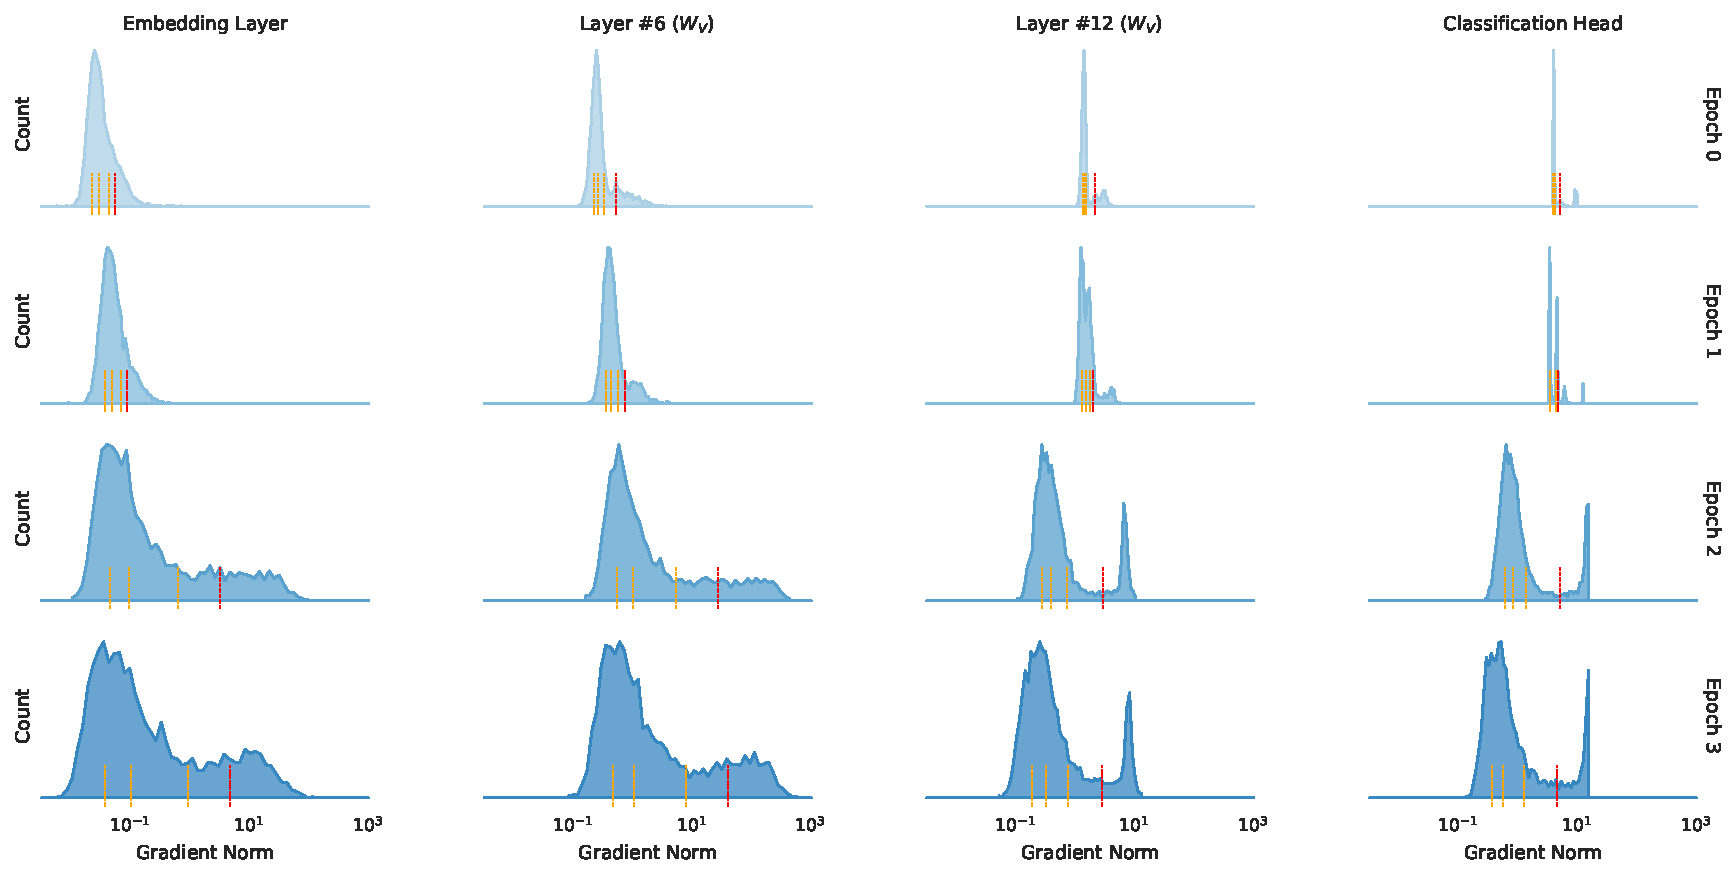
\includegraphics[width=0.95\linewidth]{files/fig/gnorm_hist_sst2_notext.pdf}
    \caption{The distribution of gradient norms of 4,096 randomly selected samples shifts across the fine-tuning procedure for the setup of SST-2 with RoBERTa-base. We show the gradient statistics of (1) the embedding layer, (2) the value matrix $W_V$ of the 6th and 12th self-attention module, (3) the final classification layer. Quantiles \{25\%, 50\% (median), 75\%, 85\%\} of the gradient norms are marked with dashed lines, from left to right.}
    \label{fig:gnorm_distribution_sst2}
\end{figure}

